\documentclass[11pt]{article}
\usepackage[margin=1in]{geometry}
\usepackage{amsmath,amssymb,booktabs,graphicx}
\usepackage[hidelinks]{hyperref}
\usepackage{xurl}
\hypersetup{pdftitle={AFTER: Digital Twins for Cyberattack and Recovery Monitoring in Industrial Robots},pdfauthor={Muhammad Usman},pdfsubject={Prediction, model mismatch and uncertainty in robotic alarm recovery}}
\DeclareMathSizes{10}{10}{8}{6}
\setlength{\emergencystretch}{2em}
\setlength{\textfloatsep}{18pt plus 2pt minus 2pt}
\renewcommand{\topfraction}{0.9}
\renewcommand{\textfraction}{0.08}
\renewcommand{\floatpagefraction}{0.8}
\makeatletter
\setlength{\@fptop}{0pt}
\setlength{\@fpsep}{18pt}
\setlength{\@fpbot}{0pt plus 1fil}
\makeatother
\newtheorem{proposition}{Proposition}
\newenvironment{proof}{\par\noindent\textit{Proof.}\ }{\hfill\textit{Q.E.D.}\par}
\title{AFTER: Digital Twins for Cyberattack and Recovery Monitoring in Industrial Robots}
\author{Muhammad Usman\\[4pt]\small COMSATS University Islamabad, Sahiwal Campus, Pakistan}
\date{}
\begin{document}
\maketitle
\begin{abstract}
A robotic digital twin may detect a motion anomaly yet give poor evidence about when the alarm should clear. Its predictor may follow unauthorized motion, or its reference may remain inaccurate after the robot recovers. We examine this problem by separating physical return from agreement with a reference model. Thirteen monitoring rules are compared on 216 synthetic episodes using the same observations and approved commands. An empirical uncertainty allowance reduces benign alarm observations from 621 to 309 relative to nominal fixed return, but allows timely clearance in only 36 of 108 detected events with physical return. Removing the allowance while keeping the entry threshold gives 140 benign alarm observations and 108 timely clearances, with no observed premature clearing. A search over 63 reference models fitted to normal data reduces the allowance by 51.27\% and 38.56\% on the harder plants, yet the overall feasibility requirement still fails. A Gaussian calculation explains why calibration noise can consume the recovery tolerance even with a perfect reference. A covariance-aware window control then meets the declared normal-feasibility criterion on 20 of 36 synthetic residual traces; temporal correlation and changing motion limit the gains from averaging. In a separate common-input inertial measurement unit (IMU) study, longer CASPER-style training lowers prediction error, but an ordinary autoregressive control remains strongest. The findings show why reduced alarm burden must be assessed alongside physical recovery, and why a clearance rule should first be checked on normal motion.
\end{abstract}
\noindent\textbf{Keywords:} digital twins; industrial robots; cyberattack detection; alarm clearance; system identification; model mismatch.

\section{Introduction}
Removing a corrupted command does not immediately undo its effect on a robot. The arm may still be displaced or moving away from its intended trajectory when the controller resumes approved commands. Clearing an alarm at that instant can hide the remaining deviation. An inaccurate nominal model creates the opposite problem: the robot recovers, but the alarm stays active because the measurements still disagree with the model. A twin used for cyberattack monitoring must therefore support decisions about both the onset and the end of abnormal motion.

Recent robotic anomaly detectors identify departures from expected behavior in motion measurements~\cite{casper,edge}, while hybrid twins combine learned components with models of robot mechanics, drives and control~\cite{hybrid}. Prediction error is useful in both settings, but its meaning depends on how the reference evolves. A predictor corrected by recent measurements may follow an unauthorized deviation and produce a small error. A reference that runs without correction may produce a large error simply because its model is inaccurate. Neither observation, by itself, tells us whether the robot has returned to authorized motion.

The question addressed here is: \emph{under model mismatch, when does discrepancy from a command-driven reference provide usable evidence for clearing a robotic attack alarm?} We assume access to noisy joint positions and velocities and a protected record of approved commands. The attacker can alter commands downstream of that record. This gives the monitor a way to predict authorized motion even when the plant executes a different command.

We first compare thirteen detection and clearance rules under a fixed attack protocol. When the uncertainty-based rule fails to clear reliably, we examine whether better references fitted to clean data resolve the problem. A Gaussian calculation and a separate residual experiment isolate the effects of measurement noise, temporal correlation and motion during the averaging window. These later analyses explain the initial failure; the original attack results remain unchanged. Appendix~\ref{app:imu} reports a separate external inertial measurement unit (IMU) prediction study that checks training adequacy under common inputs, without giving those predictors the simulation's command information.

The paper contributes an experimentally supported explanation of a failure in uncertainty-based alarm clearance. Matched comparisons identify the component responsible, while reference fitting and noise calculations explain why the difficulty persists. The window experiment shows when averaging recovers enough margin to recognize normal motion and when variation within the window prevents it. The mathematical bounds use established interval and probability arguments. AFTER is the name of this investigation; it does not denote a newly validated detector or establish an improvement over complete recent systems.

\section{Related work}
\subsection{Robotic anomaly detection and digital twins}
CASPER uses external inertial sensing and contextual information to detect anomalous industrial-arm motion~\cite{casper}. Its successor develops real-time detection with edge computing~\cite{edge}. Those inputs differ from the joint states and approved commands available in our simulation. To examine the architectures on their own modality, Appendix~\ref{app:imu} compares independent implementations on common nominal IMU observations, using causal preprocessing and simple controls. The resulting comparison concerns normal prediction. It neither reproduces the papers' attack benchmarks nor places IMU-only predictors in the same ranking as command-aware recovery monitors.

Ayankoso et al. combine kinematic and dynamic models, drive and control information, and learned uncertainty accommodation in a hybrid twin for collaborative-robot condition monitoring~\cite{hybrid}. Their work makes model fidelity and uncertainty relevant to this setting, although the benefit of an uncertainty allowance for clearing attack alarms remains a separate question. Classens et al. address structured mechanical-system identification through recursive instrumental variables and block-coordinate descent~\cite{identification}. Our finite search over autoregressive models with exogenous inputs (ARX) and finite impulse response (FIR) models uses ordinary identification methods; it is not a contribution to that identification theory.

\subsection{Uncertainty, runtime monitoring and recovery}
FAIL-Detect calibrates uncertainty-aware failure monitors from successful robot rollouts, using learned or constructed scalar signals~\cite{fail}. The full method targets imitation-learning policies and makes signal-learning and calibration choices that our experiment does not reproduce. We implement only a constant episode band on the shared discrepancy signal. This tests the thresholding principle with the same inputs as our other controls; it should not be read as an evaluation of the complete published system.

Uncertain models and observer design are already central to interval-observer fault detection~\cite{interval}. Residual bounds and dwell periods are therefore established ingredients. Our concern is their feasibility: after these allowances are applied, can the rule still recognize a return within the chosen tolerance? A rule may be conservative enough to avoid premature clearing yet leave no room to clear at all.

Kaisar et al. describe statistical detection, a kinematic twin, supervisory handover and consistency-gated recovery in a robotic-vehicle architecture~\cite{kaisar}. The available abstract directly overlaps the broad idea of twin-assisted recovery. Its full algorithm and implementation were unavailable, so an equation-level comparison remains open. Howard et al. develop time-uniform confidence sequences under explicit probabilistic assumptions~\cite{howard}. Our window control uses the simpler tools of Gaussian tails and error spending. It does not reproduce those sharper constructions or introduce a new confidence-sequence method.

The RESCUE preprint uses counterfactual robot-policy interventions to assess whether runtime alarms are worth acting on~\cite{rescue}. It distinguishes detection accuracy from the usefulness of an intervention. We also use a counterfactual, but for a narrower measurement: comparing corrupted and uncorrupted executions of the same plant to determine when a motion deviation ends. Counterfactual evaluation is thus part of the existing methodology on which this study builds. Our conclusions concern reference error, sensor noise and the tested clearance rule under the specified simulation conditions.

\section{Recovery target and clearance feasibility}
\subsection{What the monitor observes}
Let $x_t=(q_1,q_2,\dot q_1,\dot q_2)$ denote the actual state and $x_t^0$ the state of the same plant under the complete approved command history without corruption. The monitor receives $y_t=x_t+n_t$, approved commands $u_t$, and their availability indicator. A reference $r_t$ predicts the authorized trajectory. Positive scales $s_j$ are estimated from clean training observations only. Define
\begin{equation}
 \|v\|_s=\max_j |v_j|/s_j,\qquad
 d_t=\|x_t-x_t^0\|_s,\qquad c_t=\|y_t-r_t\|_s.
 \label{eq:discrepancies}
\end{equation}
The evaluator computes $d_t$; the monitor computes $c_t$. In the noise-free case, $x_t=r_t\ne x_t^0$ can give $c_t=0$ with $d_t>0$. Similarly, $x_t=x_t^0\ne r_t$ gives $d_t=0$ with $c_t>0$. A reference-discrepancy threshold consequently requires an assumption linking $r_t$ to $x_t^0$ before it can represent physical return.

\subsection{Conditional error bounds}
\begin{proposition}
If $\|x_t^0-r_t\|_s\le b_t$ and $\|n_t\|_s\le\eta_t$, then
\begin{equation}
 \max(0,c_t-b_t-\eta_t)\le d_t\le c_t+b_t+\eta_t.
 \label{eq:bound}
\end{equation}
\end{proposition}
\begin{proof}
Write $x_t-x_t^0=(y_t-r_t)-n_t-(x_t^0-r_t)$ and apply the triangle and reverse triangle inequalities. Aligned scalar errors attain the extremes, so scalar allowances alone do not generally permit tighter bounds.
\end{proof}

A sufficient return condition at tolerance $\delta$ is $c_t+b_t+\eta_t\le\delta$. This gives a simple feasibility test before any alarm experiment.
\begin{proposition}
Suppose reference and measurement errors lie in coordinate boxes with half-widths $b_{t,j}$ and $\eta_{t,j}$. Return within $\delta$ holds for every pair in those boxes exactly when
\begin{equation}
 \max_j\frac{|y_{t,j}-r_{t,j}|+b_{t,j}+\eta_{t,j}}{s_j}\le\delta.
 \label{eq:box}
\end{equation}
If $b_{t,j}+\eta_{t,j}>\delta s_j$ in any coordinate, no observation can satisfy this condition.
\end{proposition}
\begin{proof}
In each coordinate, the two admissible errors can align against the measured displacement. Their summed magnitude attains the triangle-inequality bound. The observed absolute displacement is nonnegative, yielding the infeasibility statement.
\end{proof}

These statements are conditional geometric facts. The simulated sensors have unbounded Gaussian noise, and the experiment uses an empirical discrepancy allowance rather than a verified deterministic enclosure. Specifically, the tested rule requires $c_t+b\le\delta$, where $b$ is the largest observed normal discrepancy. It is a heuristic motivated by the upper-bound form, not an implementation of a proven safety certificate. Because $b$ contains both model error and noise, interpreting it as pure reference uncertainty would be incorrect. A dwell period cannot restore feasibility when $b>\delta$.

\section{Simulation and threat model}\label{sec:simulation}
\subsection{Plant, controller and sensing}
All observations in the attack and recovery simulations are synthetic. The separate IMU prediction study uses a received public nominal recording and is described independently in Appendix~\ref{app:imu}. The simulated plant is a horizontal two-joint point-mass arm governed by
\begin{equation}
 M(q)\ddot q+C(q,\dot q)+B\dot q=\tau.
\end{equation}
Writing $a=m_2l_1l_2$ and $d=m_2l_2^2$,
\begin{align}
 M(q)&=\begin{bmatrix}(m_1+m_2)l_1^2+d+2a\cos q_2&d+a\cos q_2\\d+a\cos q_2&d\end{bmatrix},\\
 C(q,\dot q)&=a\sin q_2\begin{bmatrix}-2\dot q_1\dot q_2-\dot q_2^2\\\dot q_1^2\end{bmatrix}.
\end{align}
A proportional--derivative (PD) controller requests componentwise saturated torque
\begin{equation}
 \tau^*=\operatorname{clip}\{K_p(q^c-q)+K_d(\dot q^c-\dot q),-20,20\},
\end{equation}
with $K_p=\operatorname{diag}(18,12)$ and $K_d=\operatorname{diag}(4,3)$. Where actuator lag is present, $\dot\tau=(\tau^*-\tau)/T_a$. Nominal masses are $(1,0.8)$ kg, lengths $(0.5,0.4)$ m, and damping coefficients $(0.08,0.06)$. The nominal physics reference retains these parameters; Table~\ref{tab:plants} specifies the actual plants.

\begin{table}[htbp]\centering\small
\caption{Simulated plant configurations. Mass and damping entries multiply the nominal values; noise multiplies the stated sensor standard deviations.}\label{tab:plants}
\setlength{\tabcolsep}{5pt}
\begin{tabular}{lcccrr}\toprule
Plant & Mass factors & Damping factors & Lengths (m) & Lag (s) & Noise\\\midrule
Q1 & (1.10,0.86) & (0.80,1.20) & (0.48,0.42) & 0 & 1.0\\
Q2 & (0.88,1.15) & (1.30,0.85) & (0.53,0.37) & 0.03 & 1.0\\
Q3 & (1.16,1.06) & (0.90,1.40) & (0.46,0.43) & 0.06 & 1.5\\\bottomrule
\end{tabular}
\end{table}

Position and velocity measurements have independent, zero-mean Gaussian noise with standard deviations of 0.0005 rad and 0.002 rad/s before applying the plant multiplier. Each episode contains 1,200 observations at 50 Hz. We integrate with fourth-order Runge--Kutta, using eight substeps per observation, and check a short trajectory with actuator lag against a separate SciPy integration. That check supports numerical consistency. Physical fidelity remains limited: the model excludes gravity, contact, flexibility and thermal effects, and has not been validated against measurements from a real robot.

\subsection{Adversary and information boundaries}
The attacker acts downstream of the protected command record. It can offset an executed command, slow its progression or hold it fixed. Joint measurements remain truthful apart from sensor noise. A legitimate task change, in contrast, updates both the approved and executed command paths. The monitor's calculations use neither intervention labels nor the true state, actual plant parameters or paired counterfactual trajectory.

In the attack-study code, the monitoring routine receives a dictionary containing the complete episode. Source inspection and three replays with restricted inputs support the stated use of information, although the interface does not enforce isolation. The later normal-only study restricts the observation type itself. Both studies assume that sensing and the approved-command record are not jointly compromised, and that commissioning data are clean. Motion alone is not used to infer malicious intent.

A free reference requires the complete approved-command history. Once commands are missing, command-dependent methods remain in an unknown state for the rest of the episode, even if command availability resumes. These intervals stay in the evaluation population and count toward coverage and missed events. The persistence control does not need commands.

\section{Study I: attack detection and recovery}
\subsection{Clean commissioning and model state}
Each plant provides three known-clean commissioning episodes. Their eligible observations define the channel means and population standard deviations. Let $z_t=(y_t-\mu)/s$ denote standardized state. The ARX reference predicts
\begin{equation}
 \widehat z_t=a_0+\sum_{k=1}^{p}A_k\widetilde z_{t-k}
                    +\sum_{k=1}^{p}D_k u_{t-k},
 \label{eq:arx}
\end{equation}
where the four-component command contains approved position and velocity. For the free reference, $\widetilde z$ is its own predicted state after initialization. The one-step control instead uses measured state history. Thus the reference's maintained state is its lagged trajectory; its command-driven recurrence makes prospective predictions, while synchronization is restricted to the initial observed prefix. The following observer provides a separate measurement-corrected comparison.

Study I fixes $p=4$ and fits a ridge of $10^{-7}$ to mean normal equations, without penalizing the intercept. The first 100 observations are excluded from fitting targets. Homogeneous recursion must have spectral radius below one. The free reference starts from four observed states and receives no subsequent measurement correction. Fitted parameters remain fixed during evaluation.

\subsection{Monitoring rules and calibration}
All scores are maximum absolute standardized discrepancies. The roster includes persistence, one-step ARX, a nominal following observer, nominal free references, and learned free references. The following observer predicts before correcting its state with gains $(0.65,0.65,0.35,0.35)$. Point rules alarm when their score exceeds $h$. Hysteresis enters at the same strict exceedance and clears after ten valid observations at or below $h/2$.

Fixed-return rules instead clear after ten observations with the relevant reference discrepancy at most $\delta=0.1$. The uncertainty-return candidate requires $c_t+b\le0.1$. An entry-threshold exceedance takes priority and resets the clearance counter. Two matched ablations keep the candidate entry threshold while removing $b$ or reducing the dwell from ten samples to one.

Each plant has nineteen normal calibration episodes. Each main rule calibrates its complete alarm state machine to at most 209 alarmed observations among 20,900 eligible observations. The threshold search selects the boundary score satisfying this finite budget. The candidate allowance is the largest learned-reference discrepancy in the same calibration episodes. Calibration uses no attack labels and does not guarantee a future 1\% false-alarm rate.

The additional constant episode band takes the maximum of the nineteen whole-episode discrepancy maxima. Its rank is $\lceil(19+1)(1-0.05)\rceil=19$. This component has a different calibration objective from the main point-alarm budget. The fixed calibration grid and shifted task families do not establish the exchangeability needed for a conformal coverage guarantee. Matched-entry ablations also have their own realized calibration burdens; their role is to isolate components at an identical entry threshold.

\subsection{Frozen evaluation and metrics}
The fresh matrix crosses three new command families, three plants, seeds 17, 42 and 2026, and eight conditions, giving 216 episodes and 2,808 method/episode outcomes. The conditions are unchanged motion, authorized offset, authorized slowdown, brief unauthorized offset, persistent offset, held command, unauthorized slowdown, and offset with missing command context. The first 100 observations are processed but excluded from metrics. Corruption begins at sample 320 and ends before sample 620, except the brief offset, which lasts six samples. Offset magnitude is 0.14 rad on joint 1, slowdown rate is 0.6, and missing context spans $[320,380)$. States do not reset at intervention boundaries.

For evaluation only, a paired simulation uses the same plant and initial state with approved commands throughout. Physical return is the first post-restoration run of ten true-state observations satisfying $d_t\le0.1$, searched over five seconds. Its timestamp is the start of that qualifying window, assigned retrospectively by the evaluator. This tolerance defines a motion-effect diagnostic, not task success, collision avoidance or product quality. Nominal-reference return is retained as a secondary diagnostic.

We report unadjusted precision, recall and F1 against the command-corruption interval, average precision (AP), alarm observations and episodes on wholly benign trajectories, coverage, event overlap, fresh alarm onset, misses, premature clearing and timely clearance after physical return. An alarm already active at intervention onset counts as overlap but not fresh detection. Persistent post-intervention alarms can be false positives under interval labels while still reflecting unrecovered motion; the recovery measures expose this difference. Conditional clearance counts include only detected events with measured physical return, while all misses remain visible.

Premature clearing means an active-to-inactive transition after first detection and before the physical-return timestamp. Timely clearance means a known inactive alarm observation within five seconds of that timestamp, including alarms already inactive when physical return begins. Consequently, the timely-clearance count must be interpreted alongside premature clearing; it does not by itself show that an alarm remained active until recovery.

The predeclared primary criterion combines four requirements: at least 25\% fewer benign alarm observations than nominal fixed return; no additional missed or prematurely cleared events; at least 95\% timely clearances among detected-returned events; and benign burden no more than 10\% above learned-reference hysteresis. Models and thresholds were sealed before evaluation generation, and all score artifacts were sealed before joint outcome computation.

\subsection{Results}
The candidate failed the primary criterion. Benign alarm observations fell from 621 to 309, a reduction of 50.24\%, but only 36 of 108 detected-returned events cleared on time. The alarm overlapped 108 of 135 interventions, with 104 fresh onsets. The full comparison is in Table~\ref{tab:attack}. Figure~\ref{fig:recovery} makes the trade-off visible: the lower benign alarm count comes with poor clearance after physical return.

\begin{table}[htbp]\centering\small
\caption{Study I: complete pooled comparison. Benign counts use 89,100 observations. Overlap and fresh onset each use 135 interventions. Early counts events with premature clearing. Clear/return retains the detected-returned denominator. CP and matched-entry rows have distinct calibration interpretations.}\label{tab:attack}
\setlength{\tabcolsep}{4pt}
\begin{tabular}{lrrrrr}\toprule
Method & Benign & F1 & Overlap/fresh & Early & Clear/return \\\midrule
Persistence & 878 & 0.057 & 127/127 & 127 & 127/127 \\
ARX one-step & 792 & 0.803 & 108/108 & 108 & 108/108 \\
Following point & 794 & 0.808 & 108/108 & 108 & 108/108 \\
Following hysteresis & 993 & 0.785 & 108/108 & 108 & 108/108 \\
Nominal hysteresis & 789 & 0.713 & 108/108 & 45 & 108/108 \\
Nominal fixed return & 621 & 0.657 & 108/108 & 0 & 108/108 \\
Learned point & 819 & 0.700 & 108/108 & 18 & 108/108 \\
Learned hysteresis & 792 & 0.683 & 108/108 & 0 & 108/108 \\
Learned fixed return & 827 & 0.690 & 108/108 & 0 & 108/108 \\
Uncertainty return & 309 & 0.446 & 108/104 & 0 & 36/108 \\
Episode CP band & 0 & 0.744 & 108/108 & 75 & 108/108 \\
Matched no allowance & 140 & 0.709 & 108/108 & 0 & 108/108 \\
Matched no dwell & 20 & 0.453 & 108/108 & 0 & 36/108 \\
\bottomrule\end{tabular}

\end{table}

\begin{figure}[htbp]\centering
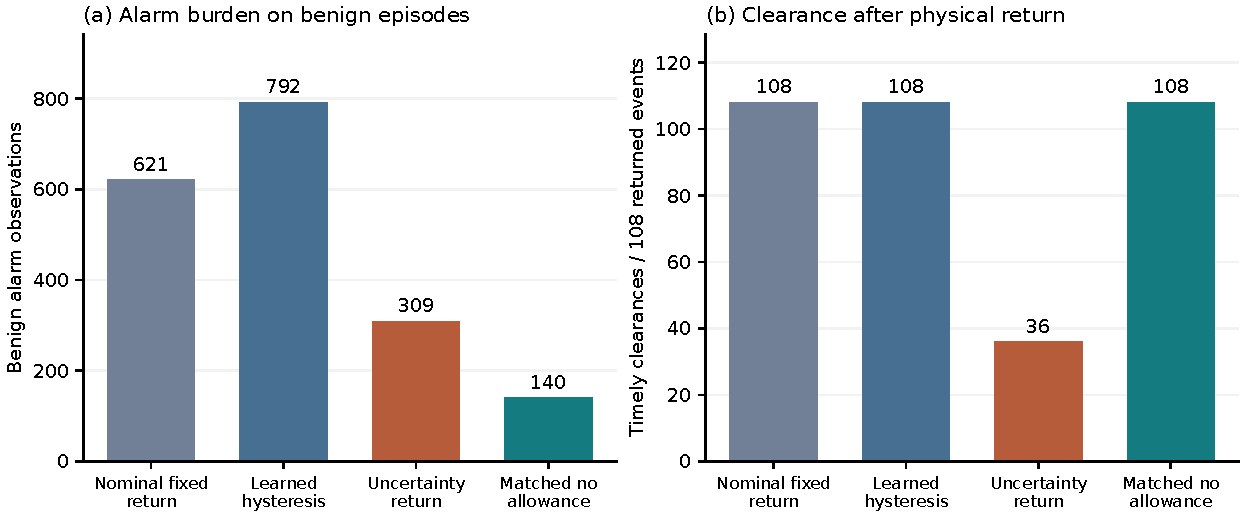
\includegraphics[width=\linewidth]{figures/recovery.pdf}
\caption{Saved Study I outcomes. All four displayed rules have zero observed premature clears, but the uncertainty-return rule fails timely clearance on 72 detected-returned events. Fewer benign alarm observations alone conceal this failure.}\label{fig:recovery}
\end{figure}

The learned-reference spectral radii are 0.95595, 0.96690 and 0.97148 for Q1--Q3. Their empirical allowances are 0.07088, 0.19149 and 0.20928. Thus Q2 and Q3 have $b>\delta$, making clearance mathematically impossible for the tested rule. Their zero benign alarm counts do not demonstrate useful recovery. All 36 timely candidate clearances come from Q1.

The matched controls locate the cause. Removing the allowance, while retaining the entry threshold, lowers benign alarms further to 140 and permits timely clearance in all 108 detected-returned events. Fresh onsets rise from 104 to 108, with no observed premature clears. Removing only the dwell period lowers benign alarms to 20 but leaves the same 72 clearing failures. The obstacle is the allowance itself; changing the waiting period cannot make an unreachable inequality hold.

Detection scores alone give a different impression. The following-observer point rule reaches F1 0.808, although it clears prematurely in all 108 detected events. The episode band produces no benign alarm observations and reaches F1 0.744, but clears prematurely in 75 events. Learned-reference hysteresis records 792 benign alarms, no premature clears and 108 timely clearances. A useful comparison therefore needs both the interval detection scores and the recovery outcomes.

All 27 missing-context interventions are missed by command-dependent methods under the unknown-history rule. Nominal-reference and paired-plant return times differ in 21 of 135 intervention episodes. The empirical allowance encloses the complete eligible counterfactual-reference discrepancy in 189 of 216 episodes, which does not establish a distribution-shift guarantee. Further point metrics, unknown coverage and alarm-episode rates appear in Appendix~\ref{app:metrics}.

\section{Study II: can better commissioning restore feasibility?}
\subsection{Finite normal-only development procedure}
Study II follows Study I and is an outcome-informed diagnosis. It uses the same three clean commissioning episodes per plant but introduces a finite model bank before generating new normal checks. ARX orders $\{4,8,16,32\}$ and FIR lengths $\{16,32,64\}$ each use ridge values $\{10^{-7},10^{-5},10^{-3}\}$. There are 21 fits per plant and 63 in total. All are eligible; no failed candidate is omitted. FIR uses the command-history terms and intercept in Equation~\ref{eq:arx}, without state-history terms.

The nineteen previously used normal calibration episodes are explicitly reused for development: the first nine select a model, the next five estimate its allowance, and the last five provide archived checks. Selection minimizes the worst episode's 99th-percentile discrepancy, breaking ties by mean standardized root mean squared error (RMSE), parameter count and model identifier. The allowance is the maximum over the five assigned episodes, or 5,500 observations. The archived checks are not relabeled independent holdouts.

Every reference receives the same 100-observation initialization prefix. A free ARX model uses the last $p$ states of that prefix, then feeds back its predictions. This differs from Study I's four-state initialization and nineteen-episode allowance. We therefore compare selected models to a matched ARX(4) within Study II. Its fitted coefficients and training transformations equal the earlier fit exactly; differences between studies' allowances cannot be attributed solely to model order.

New checks cross three previously ungenerated task families, three plants, three seeds and three normal conditions: unchanged motion, authorized offset and authorized slowdown. This gives 81 new normal episodes. Including fifteen archived checks and six recorded roles gives 576 outcomes. The selected overall model equals the selected ARX on each plant; these duplicate roles are not separate evidence.

\subsection{Feasibility criterion}
For each reference, we measure the fraction of eligible normal observations satisfying $c_t+b\le0.1$. Four diagnostic probes per episode, starting at samples 100, 320, 620 and 900, force an active latch and seek ten qualifying observations within five seconds. These probes ignore alarm-entry priority: they test the opportunity to clear during normal motion, not attack detection or actual post-attack recovery.

The predeclared admission rule requires $b<0.1$, at least 95\% feasible normal observations, and at least 95\% successful probes on every plant. A model can clear every probe yet fail the point-fraction condition. The criterion is retained unchanged after observing the results.

\subsection{Results}
The selected ARX orders are 8, 16 and 32 for Q1, Q2 and Q3, all with ridge $10^{-7}$. Mean standardized RMSE falls from 0.009477 to 0.009337 on Q1, from 0.010203 to 0.009716 on Q2, and from 0.015865 to 0.014388 on Q3. Table~\ref{tab:normal} and Figure~\ref{fig:commissioning} show that these improvements do not establish clearance feasibility across all plants.

\begin{table}[htbp]\centering\small
\caption{Study II: selected ARX versus matched ARX(4). $b_4$ and $b_\star$ are their respective allowances. Feasibility uses 29,700 new normal observations per plant. Each plant has 108 diagnostic probe starts.}\label{tab:normal}
\setlength{\tabcolsep}{4pt}
\begin{tabular}{lrrrrrr}\toprule
Plant & Order & $b_4$ & $b_\star$ & Reduction (\%) & Feasible (\%) & Clear/probes \\\midrule
Q1 & 8 & 0.0553 & 0.0553 & 0.06 & 99.82 & 108/108 \\
Q2 & 16 & 0.1469 & 0.0716 & 51.27 & 93.32 & 108/108 \\
Q3 & 32 & 0.1913 & 0.1175 & 38.56 & 0.00 & 0/108 \\
\bottomrule\end{tabular}

\end{table}

\begin{figure}[htbp]\centering
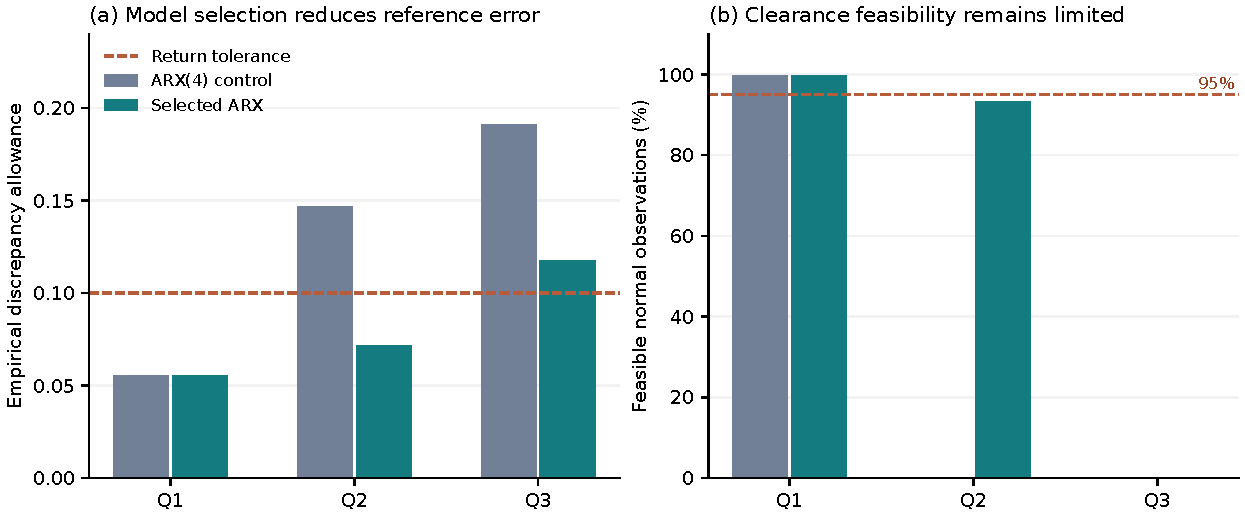
\includegraphics[width=\linewidth]{figures/commissioning.pdf}
\caption{Normal-only model development. Lower discrepancy allowances make Q2's inequality reachable, but its feasible fraction remains below 95\%. Q3's selected allowance still exceeds the return tolerance.}\label{fig:commissioning}
\end{figure}

On Q2, the allowance drops 51.27\%, from 0.146910 to 0.071592. All 108 probes clear, yet only 93.32\% of normal observations satisfy the inequality. Q3 improves by 38.56\%, from 0.191250 to 0.117495, but retains an allowance above the tolerance and clears none of its probes. Only Q1 passes all requirements. FIR(64) is selected within the FIR family on all plants but performs worse in this search. The full role comparison, including one-step ARX and command-as-state controls, is in Appendix~\ref{app:normal}. No attack evaluation of the selected replacements was conducted.

\section{Noise allocation explains the remaining obstruction}
The remaining normal-motion failure raises a simple question: would a perfect reference solve it? To examine this, consider a hypothetical free reference $r_t=x_t^0$ under normal motion, retaining the simulator's independent Gaussian measurement noise and fixed training scales. Let $\nu_j=\sigma_j/s_j$. The scalar noise discrepancy has distribution
\begin{equation}
 F(x)=\Pr\{\|n_t\|_s\le x\}
     =\prod_{j=1}^{4}\operatorname{erf}\!\left(\frac{x}{\sqrt{2}\nu_j}\right),
 \qquad x\ge0.
\end{equation}
For an empirical allowance $B$ equal to the maximum of $N$ independent calibration discrepancies,
\begin{equation}
 \Pr(B\le b)=F(b)^N.
\end{equation}
Conditioned on $B$, a new normal observation satisfies the rule with probability $F(\delta-B)$, taking $F(x)=0$ for $x<0$. A population feasibility of at least $\gamma$ therefore requires
\begin{equation}
 B\le\delta-F^{-1}(\gamma),\qquad
 \Pr\{F(\delta-B)\ge\gamma\}
 =F\!\left(\delta-F^{-1}(\gamma)\right)^N.
 \label{eq:noiseprob}
\end{equation}
The tolerance is being shared between two noisy quantities. Increasing $N$ makes the calibration maximum stochastically larger and leaves less margin for the next observation. A larger calibration sample therefore does not automatically help this particular rule. Better reference fitting cannot remove the contribution from measurement noise.

\begin{table}[htbp]\centering\small
\caption{Conditional perfect-reference diagnostic with $N=5{,}500$, $\delta=0.1$ and $\gamma=0.95$. The final column is the probability that a noise-only calibration maximum leaves enough margin for 95\% population feasibility.}\label{tab:noise}
\begin{tabular}{lrrr}\toprule
Plant & $F^{-1}(0.95)$ & $\delta-F^{-1}(0.95)$ & Margin probability \\\midrule
Q1 & 0.028251 & 0.071749 & 0.999828 \\
Q2 & 0.027914 & 0.072086 & 0.999897 \\
Q3 & 0.041737 & 0.058263 & $2.19\times10^{-9}$ \\
\bottomrule\end{tabular}

\end{table}

For Q3, the single-observation noise quantile is 0.041737, leaving an allowable calibration maximum of only 0.058263. Equation~\ref{eq:noiseprob} gives approximately $2.19\times10^{-9}$. The corresponding probabilities for Q1 and Q2 exceed 0.9998. Two numerical implementations agree on these values.

The calculation conditions on the declared independent Gaussian noise and the fitted training scales. It is a population statement about the clearance inequality, not the probability of passing a finite empirical check, a dwell-time calculation, or an estimate across real robots. It was added after Study II and changed no selected model, tolerance or criterion. It explains why the maximum-plus-discrepancy construction can remain unusable even when reference error is removed; it does not establish that all uncertainty-aware recovery decisions fail.

\section{Study III: covariance-aware return bounds}\label{sec:window}
\subsection{A standard control for current deviation}
Averaging offers a way to reduce noise, but a clearance decision concerns the robot's motion now. The following control accounts for both effects. It separates reference bias from measurement noise instead of treating an empirical residual maximum as a model-error bound. For a dimensionless channel $j$, write
\begin{equation}
 e_{t,j}=v_{t,j}+\beta_{t,j}+\epsilon_{t,j},
 \qquad |\beta_{t,j}|\le B_j,\quad |v_{t,j}-v_{t-1,j}|\le L_j,
 \label{eq:decomposition}
\end{equation}
where $v$ is physical deviation from the nominal response, $\beta$ is reference bias, and $\epsilon$ is measurement noise. Assume a stationary zero-mean Gaussian AR(1) noise process with marginal standard deviation $\sigma_j$ and correlation $0\le\rho_j<1$. The variance of a mean over $m$ consecutive noise observations is
\begin{equation}
 V_{m,j}=\frac{\sigma_j^2}{m^2}
 \left[m+2\sum_{k=1}^{m-1}(m-k)\rho_j^k\right].
 \label{eq:covariance}
\end{equation}
Independence gives $V_{m,j}=\sigma_j^2/m$. Positive serial correlation reduces the effective averaging benefit.

Let $\mathcal M$ contain $K$ fixed windows, let $d$ be the number of channels, and allocate $\alpha_t=6\alpha/(\pi^2t^2)$ using a global clock that does not restart at alarms. Define
\begin{equation}
 U_{t,j}(m)=|\overline e_{t,j}(m)|+B_j
 +\sqrt{2V_{m,j}\log(2dK/\alpha_t)}
 +\frac{L_j(m-1)}{2}.
 \label{eq:windowbound}
\end{equation}
The last term covers motion during the window. Without it, a small average deviation could be mistaken for a small current deviation.

\begin{proposition}
Under the stated Gaussian covariance, bias and increment assumptions, with probability at least $1-\alpha$, $|v_{t,j}|\le U_{t,j}(m)$ simultaneously for every channel, complete registered window and prospective time within a trace. Consequently, the decision
\begin{equation}
 \min_{m\in\mathcal M}U_{t,j}(m)\le\delta_j\qquad(j=1,\ldots,d)
 \label{eq:certificate}
\end{equation}
certifies coordinatewise return on that simultaneous event.
\end{proposition}
\begin{proof}
The Gaussian mean has variance $V_{m,j}$, so its two-sided tail at the square-root term in Equation~\ref{eq:windowbound} is at most $\alpha_t/(dK)$. Sum over channels, registered windows and times, using $\sum_{t=1}^{\infty}\alpha_t=\alpha$. Window overlap and cross-channel dependence do not invalidate this union bound. Finally, $|\overline\beta|\le B_j$ and
$|v_{t,j}-\overline v_{t,j}(m)|\le m^{-1}\sum_{k=0}^{m-1}kL_j=L_j(m-1)/2$.
The triangle inequality gives the result. Each coordinate may use a different minimizing window because all bounds hold simultaneously.
\end{proof}

This control follows from elementary probability bounds and makes no new claim in time-uniform inference. The error allocation is conservative, and the guarantee holds only under the supplied covariance and deterministic bounds. An unknown or invalid observation invalidates the affected windows without restarting the clock. Failure to obtain a certificate leaves return uncertain; it does not generate an attack alarm. Arbitrary colored, heavy-tailed or nonstationary noise is outside the model.

\subsection{Prospective residual experiment}
The diagnostic fixes $d=4$, $\mathcal M=\{1,41,201\}$, $\alpha=0.05$, $\delta_j=0.1$ and $B_j=0.01$. Four $(\sigma,\rho)$ settings are $(0.03,0)$, $(0.06,0)$, $(0.03,0.8)$ and $(0.06,0.95)$, with channel standard-deviation multipliers $(1,0.8,1.1,0.9)$. For phases $\phi_j=(0,0.4,0.8,1.2)$, bias is $0.01\cos(0.003t+\phi_j)$. The physical-deviation signals are zero, $0.02\sin(0.004t+\phi_j)$, and $0.02\sin(0.04t+\phi_j)$, termed settled, slow and faster variation. They always lie within tolerance. The corresponding increment bound is $L_j=2a|\sin(\omega/2)|$, derived from the declared amplitude and frequency.

Each trace contains 1,200 samples, with the first noise value drawn from the stationary marginal. Seeds 17,42,2026 produce three independent innovation arrays reused across settings, giving 36 paired constructed traces rather than 36 independent acquisitions. The common reporting support is samples 201--1,200, or 1,000 endpoints per trace. The error statement is marginal per trace; no simultaneous 95\% guarantee across this whole matrix is claimed.

All four valid controls---the three fixed windows and their simultaneous envelope---receive identical residuals and parameter bounds. Two deliberately misspecified controls set $\rho=0$ for the 41- and 201-sample windows. Every variant and all 216 outcomes are retained. The criterion requires at least 95\% of common endpoints certified on every trace by the envelope. Parameters and conditions were recorded before generating outcomes; none was changed afterward.

The generator constructs these residual signals directly; it does not run the robot dynamics of Section~\ref{sec:simulation}. It also supplies the noise, bias and increment bounds. This lets the experiment isolate their mathematical effects, but leaves open how an operational monitor would obtain those bounds from commissioning data. The diagnostic contains no attacks, threshold fitting or model learning, and measures no post-attack recovery delay.

\subsection{Results and implications}
The envelope passes on 20 of 36 traces and therefore fails the overall normal-feasibility requirement. Table~\ref{tab:window} includes every condition group and its range across seeds; Figure~\ref{fig:window} shows the lowest fraction in each group. The instantaneous control certifies no endpoints. Averaging helps in several settings, but taking the longest window or assuming independent noise does not work uniformly.

\begin{table}[htbp]\centering\small
\caption{Study III: simultaneous-envelope certificates on normal synthetic residuals. Each range spans the three seeds, each with 1,000 common endpoints. Passing requires at least 95\% on each trace.}\label{tab:window}
\setlength{\tabcolsep}{5pt}
\begin{tabular}{llrr}\toprule
Noise setting & Deviation profile & Certificates (\%) & Passes \\\midrule
Independent, low & Settled & 100.0--100.0 & 3/3 \\
Independent, low & Slow variation & 100.0--100.0 & 3/3 \\
Independent, low & Faster variation & 100.0--100.0 & 3/3 \\
Independent, high & Settled & 100.0--100.0 & 3/3 \\
Independent, high & Slow variation & 100.0--100.0 & 3/3 \\
Independent, high & Faster variation & 17.2--25.6 & 0/3 \\
Correlated, low & Settled & 100.0--100.0 & 3/3 \\
Correlated, low & Slow variation & 85.8--100.0 & 2/3 \\
Correlated, low & Faster variation & 0.0--0.0 & 0/3 \\
Correlated, high & Settled & 0.0--0.0 & 0/3 \\
Correlated, high & Slow variation & 0.0--0.0 & 0/3 \\
Correlated, high & Faster variation & 0.0--0.0 & 0/3 \\
\bottomrule\end{tabular}

\end{table}

\begin{figure}[htbp]\centering
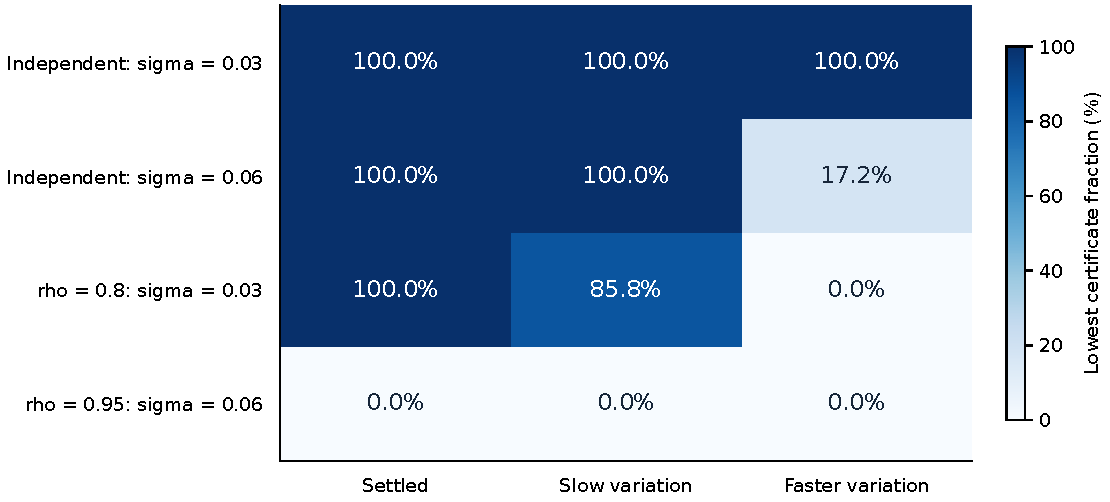
\includegraphics[width=0.88\linewidth]{figures/window_feasibility.pdf}
\caption{Lowest certificate fraction across seeds for each synthetic residual condition. All physical-deviation signals are within tolerance. A certificate establishes only the conditional bound in Equation~\ref{eq:certificate}; low coverage is not an attack-detection result.}\label{fig:window}
\end{figure}

For independent low noise with faster variation, window 41 certifies every endpoint, whereas window 201 certifies none. The longer window's drift allowance consumes its noise benefit. Under correlated low noise and slow variation, the envelope's fractions are 100\%, 85.8\% and 100\%: their 95.27\% average does not satisfy the all-traces criterion. At $\rho=0.95$ and $\sigma=0.06$, no valid control certifies any common endpoint, even for the settled profile. The misspecified 201-sample control would certify 91.53\% on average for that settled profile, but its uncertainty claim no longer follows from the actual covariance.

There are no observed coverage violations, but all the constructed deviations lie within tolerance. These traces cannot estimate rare unsafe-clearing risk or establish performance near the tolerance boundary. The experiment instead exposes the competing effects of window length: more averaging reduces noise uncertainty while increasing the allowance for current-state variation. Choosing a window after seeing its outcome would not resolve that conflict. The decision needs defensible information about noise and motion.

The diagnostic completed in 0.565 s wall time and 0.459 s CPU time, with 39.81 MiB sampled peak memory and 11.07 MiB of outputs. Twenty synthetic software checks and 2,665 saved-artifact checks support its implementation. These costs cover the entire small diagnostic and cannot be interpreted as robot deployment latency.


\section{Discussion}
The central failure was easy to miss if judged only by benign alarm counts. The candidate produced fewer such alarms, yet on two plants its clearing condition could never be satisfied. Removing the uncertainty allowance under the same entry threshold gave better outcomes. In this experiment, the added allowance did not earn its place in the rule. The result also separates questions that an interval detection score combines poorly: whether an attack is detected, whether its physical effect remains, and whether the monitor can recognize recovery.

Better commissioning helps, but only to a point. Longer ARX histories lower normal prediction error and make Q2's clearing condition reachable. Q3 still fails. The perfect-reference calculation explains why fitting alone is insufficient: the empirical maximum contains measurement noise as well as model error. Adding that maximum to another noisy residual can use up the tolerance even when there is no physical deviation. Reference bias and measurement noise therefore need separate treatment.

A recovery monitor should first specify what return means and which observations it can trust. The next check is whether its clearing condition is reachable during normal motion. Only then is it useful to examine detection, alarm persistence and recovery together. Algebraic reachability, the fraction of feasible observations and successful dwell probes answer different parts of that question; none alone establishes a safe reset policy. Any replacement should also be tested against ordinary statistical estimation, averaging and noise-aware observers, since these already address parts of the problem.

Study III shows what averaging can and cannot repair. Windowed bounds certify some normal residuals that the instantaneous bound cannot certify. With stronger correlation or faster variation within tolerance, that advantage disappears. A longer window reduces the noise term but increases the allowance for change between the window average and the current state. Assuming independent noise when it is correlated makes some certificate fractions look better while removing their statistical justification. Here the generator supplied the uncertainty parameters; an operational monitor would have to justify them from commissioning observations and knowledge of the plant.

The choice of recovery reference matters as well. Nominal-reference and actual-plant return times disagree in 21 intervention episodes. If the detector's nominal model also defines the evaluation target, model mismatch can be mistaken for a lingering attack effect. The simulation separates these trajectories within the model. A physical deployment would not have that exact counterfactual, so the recovery target would carry uncertainty of its own.

\subsection{Evidence scope}
The simulated motion comes from three plant configurations in one simulator. Repeating them with different noise seeds does not provide independent robot acquisitions. Geometry, damping, lag and noise also vary together, so a subgroup difference cannot be attributed to one of those factors alone. The study covers neither contact-rich tasks nor manufacturing-process changeovers, field attacks or hardware measurements. The chosen return tolerance has no established safety interpretation.

The attack comparison tests controls with common information and a restricted calibration component. It does not reproduce three complete recent methods. The IMU appendix adds executable architectural comparisons, but uses an already exposed normal-development prefix; the compact models still reach the epoch limit, and correspondence to the original published runs remains unresolved. These input and protocol differences prevent a fair overall ranking of external-IMU baselines and protected-command monitors. The matched internal ablations are informative within that narrower scope.

The order of the studies limits what can be claimed. Study I evaluates a fixed candidate prospectively. Study II uses its outcome to motivate new normal-task checks, followed by a conditional mathematical explanation. Study III was specified before its residual traces were generated, but grew out of those earlier failures and remains a simplified diagnostic. Its three noise realizations are reused across settings. All these conditions are now exposed, so a redesign based on them would need a new prospective evaluation for confirmation.

\section{Conclusion}
A smaller prediction error does not settle when an attack alarm should clear. In our simulation, the empirical uncertainty allowance halves benign alarm observations relative to nominal fixed return, yet prevents timely clearance in two-thirds of detected-returned events. The matched rule without the allowance performs better. Fitting more accurate references helps, but does not restore feasibility on every plant. Calibration noise can consume the return margin even with a perfect reference, and averaging introduces a further trade-off with uncertainty about current motion. The window control meets its criterion on 20 of 36 constructed normal traces. In the separate IMU study, ordinary autoregression also remains a strong control after longer convolutional neural network (CNN) training. These findings support checking normal-return feasibility and uncertainty assumptions before interpreting a lower alarm count as an improvement. They do not establish a universal reset policy or superiority over CASPER.

\appendix
\section{Command trajectories and reproducibility}
For phase $\theta(s)$, amplitudes $a_1,a_2$ and offset $\phi$,
\begin{align}
 q_1^c&=a_1\sin\theta+0.025\sin(2.3\theta),\\
 q_2^c&=a_2\sin(\theta+\phi)+0.018\sin(1.7\theta).
\end{align}
Velocities are analytic derivatives multiplied by the causal time-warp rate. Study I tasks E, F and G use, respectively,
\begin{align*}
 E:&\quad \theta=0.63s,\quad (a_1,a_2,\phi)=(0.31,0.35,0.8),\\
 F:&\quad \theta=0.38s+0.008s^2,\quad (0.26,0.40,1.2),\\
 G:&\quad \theta=0.83s+0.18\sin(0.31s),\quad (0.36,0.32,0.4).
\end{align*}
Study II tasks H, I and J use the same respective phase forms, with base rates 0.52, 0.45 and 0.93, and amplitude/offset tuples $(0.28,0.37,1.4)$, $(0.34,0.33,0.7)$ and $(0.25,0.38,1.0)$. Authorized slowdown retains accumulated phase delay; unauthorized slowdown rejoins the approved schedule on restoration.

Commissioning episodes use phase rates 0.35, 0.7 and 1.1, with amplitudes $(0.22+0.04i,0.34-0.025i)$ and offset $0.5+0.3i$, $i=0,1,2$. They respectively use unchanged, authorized-offset and authorized-slowdown conditions. Normal calibration episode $i=0,\ldots,18$ uses rate $0.32+0.047i$, amplitudes $(0.23+0.012(i\bmod7),0.29+0.013(i\bmod9))$ and offset $0.4+0.06(i\bmod11)$, cycling through these benign conditions.

The retained reproducibility package contains configurations, source/input hashes, all fitted candidates, selection and calibration records, score seals, complete outcomes, dependency versions and resource logs. Study I is recorded as recovery v0.8; Study II as commissioning v0.9; Study III as return-bound v0.12; and the separate IMU study as CASPER convergence v0.11. They use Python 3.12.15 and NumPy 1.26.4 in isolated project environments; the CNN study additionally uses TensorFlow 2.16.2. Tables and figures are generated from saved result files, without fitting or simulation during manuscript production.

Study I completed in 229.20 s supervised wall time and 228.07 s worker CPU time, with 167.25 MiB sampled peak memory and 118.32 MiB of outputs. The worker's process-lifetime peak was 217.41 MiB. Study II used 14.75 s wall and 14.30 s CPU, with 113.97 MiB sampled peak memory, 117.66 MiB worker peak and 28.02 MiB of outputs. These are whole-run measurements, not per-observation deployment latency.

Fourteen synthetic checks preceded Study I; 23 preceded Study II. Post-run audits passed 9,610 and 10,293 checks, respectively, covering hashes, fitted artifacts, score alignment and independently recomputed metrics. The initial Study I launch failed before worker initialization because process monitoring was blocked. The initial Study II attempt stopped on a reporting-key collision after selection and before fresh generation. A separately recorded repair preserved byte-identical fits and selection before continuation. These attempts and the numerical replay environment are retained in the package. Software checks support reproducibility rather than physical validation.

\section{Separate common-input IMU prediction study}\label{app:imu}
\subsection{Release, chronology and permitted information}
This study compares normal prediction when every model receives the same inputs. Its results are reported separately from the command-aware attack comparison. We use the received author-linked CASPER-1-and-2 provider-v2 nominal file \texttt{IMU\_10Hz.csv}, obtained from the \href{https://www.kaggle.com/datasets/hkayan/industrial-robotic-arm-imu-data-casper-1-and-2}{public provider listing}. Its SHA-256 is\nopagebreak[4]
\begin{center}\small\url{1221df9be80c229969f3f21f820837e68ad28f4ccb3949bf4013f00d6d69d62c}.\end{center}
This file differs from the original CASPER-v3 archive, and its exact correspondence to the original paper's runs remains unresolved. It contains nine channels: X/Y/Z measurements from an accelerometer, gyroscope and magnetometer. We could not resolve the timestamp units or whether they record acquisition or arrival. The filename is therefore insufficient evidence for reporting elapsed time or detection delay.

Training uses numeric rows 219--9184 and development uses rows 9185--12006, indexed from zero. The split precedes a trailing width-20 median filter. Each partition loses its first 19 filtered warmup observations. Training alone supplies the channel means and population standard deviations; constant or nonfinite channels are rejected. The clock must increase strictly, with no gap greater than five times the training median increment. All models use the same eligible targets after 755 history observations: 8,192 training and 2,048 development targets. The development target rows are 9959--12006 inclusive. A 755-residual aggregation leaves 1,294 aligned development endpoints. This prefix had already been used for development and is not an independent final test.

\subsection{Architectures, fitting and model selection}
The CASPER-style architecture follows the corrected manuscript's four valid one-dimensional convolutions, each with 32 filters, kernel size five and ReLU activation. Max pooling with width three follows each pair; flattening and a nine-output dense layer give 39,977 parameters for history length 755. The compact Edge-style architecture has two valid convolutions with eight filters and kernel size three, followed by width-three pooling and a nine-output dense layer: 1,369 parameters for history length 45. Both are independently written architectural implementations under a modified protocol. A zero-initialized output layer, batch size 64 and the present causal preprocessing are disclosed implementation choices, not proof of correspondence to a published checkpoint.

Training uses mean squared error (MSE), Adamax at learning rate $10^{-3}$, chronological minibatches without shuffling, and seeds 17,42,2026. All models start afresh for this longer study; optimizer state was not transferred from the short pilot. The maximum is 100 epochs. A development improvement greater than $10^{-6}$ selects a checkpoint; five epochs without such improvement stop training. Per-fit CPU admission is limited to 240 seconds, with total ceilings of 1,200 seconds wall and 900 seconds CPU. No attack labels select training duration, model weights or score formulas.

Training-mean, persistence and AR(4) controls use the same target observations. The AR control fits standardized channels with ridge $10^{-3}$ on mean normal equations, leaving the intercept unpenalized. The reported MSE averages squared error over the nine standardized target channels and 2,048 development endpoints. Mean, persistence and AR run once; all stochastic seeds are reported separately.

\begin{table}[htbp]\centering\small
\caption{Normal-development prediction on the common filtered IMU prefix. Epoch columns show completed and selected epochs. All nine outcomes are retained.}\label{tab:imu}
\setlength{\tabcolsep}{5pt}
\begin{tabular}{lrrrl}\toprule
Predictor & Seed & MSE & Epochs & Stopping \\\midrule
Training mean & -- & 1.073987 & -- & Closed form \\
Persistence & -- & 0.019432 & -- & Closed form \\
AR(4) & -- & 0.006074 & -- & Closed form \\
CASPER-style CNN & 17 & 0.017703 & 27/22 & Patience \\
CASPER-style CNN & 42 & 0.017451 & 27/22 & Patience \\
CASPER-style CNN & 2026 & 0.017458 & 27/22 & Patience \\
Edge-style CNN & 17 & 0.044730 & 100/100 & Epoch limit \\
Edge-style CNN & 42 & 0.043451 & 100/100 & Epoch limit \\
Edge-style CNN & 2026 & 0.042700 & 100/100 & Epoch limit \\
\bottomrule\end{tabular}

\end{table}

\subsection{Results and interpretation}
Longer training lowers the CASPER-style errors. Every seed stops under the declared patience rule after 27 epochs and selects epoch 22, with MSE 0.017451--0.017703. These errors are 46.11--58.12\% below the corresponding short-pilot values. The compact models all reach 100 epochs while still improving; their MSE 0.042700--0.044730 remains limited by the training budget. AR(4) gives the lowest error on this prefix, 0.006074. Figure~\ref{fig:imu} includes the learning curve for every neural seed.

\begin{figure}[htbp]\centering
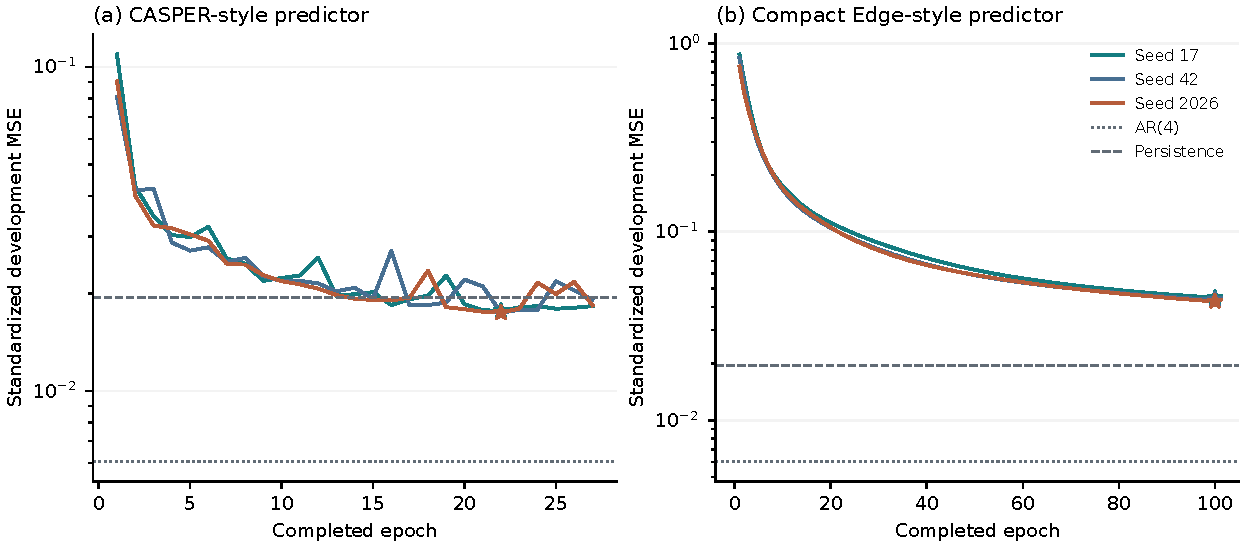
\includegraphics[width=\linewidth]{figures/imu_learning_curves.pdf}
\caption{Normal-development learning curves from the saved training records. Local patience stopping supports greater training adequacy for the CASPER-style architecture; the compact models remain limited by the epoch ceiling. Horizontal control lines refer to the same filtered targets.}\label{fig:imu}
\end{figure}

These results apply to the filtered normal prefix. Median filtering changes the prediction task and introduces dependence, so the autoregressive advantage cannot be assumed to hold for unfiltered attack detection. The patience rule establishes when these runs stopped, not a global optimum, convergence on a representative full dataset or reproduction of the published experiments. This study computes no attack threshold, F1 or recovery score and performs no test-label optimization. Lower normal MSE alone is insufficient evidence of better cyberattack detection.

The run used 764.794 s wall time, 753.252 s CPU, 553.05 MiB sampled peak memory and 2.68 MiB of outputs. Seventeen pre-run synthetic checks and 3,754 fresh-process artifact checks covered checkpoint reloads, score alignment and source identities. The hardware was the same macOS arm64 workstation; process threads and actual budgets are retained in provenance. No neural model was refitted while preparing this manuscript.


\section{Additional attack metrics}\label{app:metrics}
Table~\ref{tab:metrics} uses unadjusted command-corruption labels. AP evaluates scalar-score ranking, not clearance quality. Unknown observations remain eligible, cannot count as detected attacks, and receive AP score $-1$, below valid nonnegative scores. Known coverage excludes unknown states. Alarm episodes per hour divide starts on wholly benign episodes by their eligible duration. Point rules can have frequent alarm starts despite a small alarmed-point fraction.

\begin{table}[htbp]\centering\small
\caption{Study I: additional metrics. All methods have 237,600 eligible observations and 135 intervention events.}\label{tab:metrics}
\setlength{\tabcolsep}{3pt}
\begin{tabular}{lrrrrrr}\toprule
Method & Precision & Recall & AP & Episodes/h & Missed & Known (\%) \\\midrule
Persistence & 0.203 & 0.033 & 0.130 & 480.8 & 8 & 100.0 \\
ARX one-step & 0.868 & 0.748 & 0.770 & 1426.3 & 27 & 90.0 \\
Following point & 0.878 & 0.747 & 0.770 & 793.9 & 27 & 90.0 \\
Following hysteresis & 0.841 & 0.735 & 0.770 & 99.0 & 27 & 90.0 \\
Nominal hysteresis & 0.706 & 0.719 & 0.587 & 84.8 & 27 & 90.0 \\
Nominal fixed return & 0.656 & 0.658 & 0.587 & 48.5 & 27 & 90.0 \\
Learned point & 0.658 & 0.748 & 0.589 & 1054.5 & 27 & 90.0 \\
Learned hysteresis & 0.628 & 0.747 & 0.589 & 62.6 & 27 & 90.0 \\
Learned fixed return & 0.641 & 0.747 & 0.589 & 115.2 & 27 & 90.0 \\
Uncertainty return & 0.318 & 0.747 & 0.589 & 26.3 & 27 & 90.0 \\
Episode CP band & 0.742 & 0.746 & 0.589 & 0.0 & 27 & 90.0 \\
Matched no allowance & 0.675 & 0.747 & 0.589 & 28.3 & 27 & 90.0 \\
Matched no dwell & 0.325 & 0.747 & 0.589 & 28.3 & 27 & 90.0 \\
\bottomrule\end{tabular}

\end{table}

\section{Complete normal-reference comparison}\label{app:normal}
Table~\ref{tab:normalall} retains all distinct reference roles. Mean RMSE is computed over standardized state channels and averaged across episodes. Selected-reference and selected-ARX roles are identical and appear once. FIR models receive only past approved commands, while the one-step ARX uses observed history. Forced-latch clearance counts are normal diagnostics and must not be read as attack-recovery success.

\begin{table}[htbp]\centering\small
\caption{Study II: all distinct roles on the new normal tasks. Every row uses 29,700 eligible observations and 108 probes.}\label{tab:normalall}
\setlength{\tabcolsep}{4pt}
\begin{tabular}{llrrrr}\toprule
Plant & Reference & RMSE & Allowance & Feasible (\%) & Clear/probes \\\midrule
Q1 & ARX(4), free & 0.00948 & 0.0553 & 99.80 & 108/108 \\
Q1 & Selected ARX, free & 0.00934 & 0.0553 & 99.82 & 108/108 \\
Q1 & Selected FIR & 0.01211 & 0.2322 & 0.00 & 0/108 \\
Q1 & ARX(4), one-step & 0.00976 & 0.0649 & 97.92 & 108/108 \\
Q1 & Command as state & 0.09584 & 2.1344 & 0.00 & 0/108 \\
Q2 & ARX(4), free & 0.01020 & 0.1469 & 0.00 & 0/108 \\
Q2 & Selected ARX, free & 0.00972 & 0.0716 & 93.32 & 108/108 \\
Q2 & Selected FIR & 0.01693 & 0.3971 & 0.00 & 0/108 \\
Q2 & ARX(4), one-step & 0.01036 & 0.1211 & 0.00 & 0/108 \\
Q2 & Command as state & 0.10423 & 2.1528 & 0.00 & 0/108 \\
Q3 & ARX(4), free & 0.01586 & 0.1913 & 0.00 & 0/108 \\
Q3 & Selected ARX, free & 0.01439 & 0.1175 & 0.00 & 0/108 \\
Q3 & Selected FIR & 0.02215 & 0.4596 & 0.00 & 0/108 \\
Q3 & ARX(4), one-step & 0.01573 & 0.1807 & 0.00 & 0/108 \\
Q3 & Command as state & 0.11251 & 2.2058 & 0.00 & 0/108 \\
\bottomrule\end{tabular}

\end{table}
\section*{Data and code availability}
The attack/recovery episodes and residual traces are synthetic. The separate prediction study uses the author-linked CASPER-1-and-2 nominal release identified in Appendix~\ref{app:imu}; original recordings remain subject to their provider's terms. Source code, configurations, hashes, fitted artifacts and complete outcomes are retained in the research reproducibility package. No public release of that package has been made. The manuscript source package contains the figure and table assets used in this article and does not redistribute raw recordings.

\section*{Funding}
This research received no funding.

\section*{Competing interests}
The author declares no competing interests.

\section*{Declaration of AI assistance}
OpenAI Codex assisted literature checking, study design, programming, experiment execution, artifact verification and manuscript preparation. Numerical tables and figures were generated with Python and Matplotlib from saved experimental artifacts. No generative image model was used to produce the scientific figures.

\begingroup\interlinepenalty=10000
\begin{thebibliography}{9}
\bibitem{casper} H. Kayan, R. Heartfield, O. Rana, P. Burnap, and C. Perera. CASPER: Context-Aware IoT Anomaly Detection System for Industrial Robotic Arms. \emph{ACM Transactions on Internet of Things}, 5(3), Article 18, 2024. \url{https://doi.org/10.1145/3670414}.
\bibitem{edge} H. Kayan, R. Heartfield, O. Rana, P. Burnap, and C. Perera. Real-Time Anomaly Detection for Industrial Robotic Arms Using Edge Computing. \emph{IEEE Internet of Things Journal}, 12(15):29696--29712, 2025. \url{https://doi.org/10.1109/JIOT.2025.3569780}.
\bibitem{hybrid} S. Ayankoso, E. Kaigom, H. Louadah, H. Faham, F. Gu, and A. Ball. A Hybrid Digital Twin Scheme for the Condition Monitoring of Industrial Collaborative Robots. \emph{Procedia Computer Science}, 232:1099--1108, 2024. \url{https://doi.org/10.1016/j.procs.2024.01.108}.
\bibitem{identification} K. Classens, R. A. Gonz\'alez, and T. Oomen. Recursive identification of structured systems: An instrumental-variable approach applied to mechanical systems. \emph{European Journal of Control}, 84:101238, 2025. \url{https://doi.org/10.1016/j.ejcon.2025.101238}.
\bibitem{fail} C. Xu, T. K. Nguyen, E. Dixon, C. Rodriguez, P. Miller, R. Lee, P. Shah, R. A. Ambrus, H. Nishimura, and M. Itkina. Can We Detect Failures Without Failure Data? Uncertainty-Aware Runtime Failure Detection for Imitation Learning Policies. \emph{Robotics: Science and Systems XXI}, 2025. \url{https://doi.org/10.15607/RSS.2025.XXI.073}.
\bibitem{interval} J. Meseguer, V. Puig, T. Escobet, and J. Saludes. Observer gain effect in linear interval observer-based fault detection. \emph{Journal of Process Control}, 20(8):944--956, 2010. \url{https://doi.org/10.1016/j.jprocont.2010.06.017}.
\bibitem{kaisar} H. Kaisar, M. Rehan, I. Ahmed, M. Bilal, and M. Khalid. A Digital Twin-Based Cybersecurity Architecture for FDI Anomaly Detection and Isolation in Next Generation Robotic Vehicles. \emph{IEEE Open Journal of the Communications Society}, 7:12709--12728, 2026. \url{https://doi.org/10.1109/OJCOMS.2026.3739185}.
\bibitem{howard} S. R. Howard, A. Ramdas, J. McAuliffe, and J. Sekhon. Time-uniform, nonparametric, nonasymptotic confidence sequences. \emph{The Annals of Statistics}, 49(2):1055--1080, 2021. \url{https://doi.org/10.1214/20-AOS1991}.
\bibitem{rescue} D. Ahmedt-Aristizabal, A. Khamis, M. A. Armin, and L. Petersson. RESCUE: Is This Alarm Worth Acting On? Counterfactual Evaluation of VLA Runtime Monitors. \emph{arXiv preprint} arXiv:2610.13516v1, 2026. \url{https://arxiv.org/abs/2610.13516v1}.
\end{thebibliography}
\endgroup
\end{document}
